\documentclass[multiple,border=12pt]{standalone}
\usepackage{tikz}
\begin{document}
% Where does a ROTATED node's ink land when `anchor=` names one of its anchors? pgf turns the node
% and then puts the TURNED anchor on the point. The fill prices the rectangle, the dot is the point
% and `REF` at (-2,0) fixes the user scale. One page per case, read back by
% _work/probe100h_rot_anchors.py.
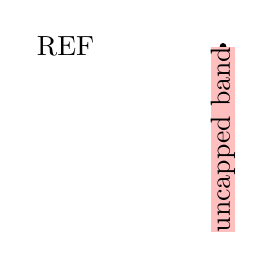
\begin{tikzpicture}[x=1cm,y=1cm]
  \node (A) at (-2,0) {REF};
  \fill (0,0) circle (1.2pt);
  \node[anchor=east,rotate=90,fill=red!25,inner sep=0pt] at (0,0) {uncapped band};
\end{tikzpicture}
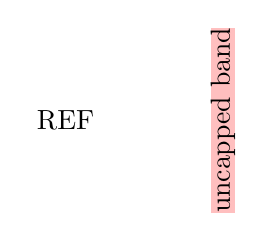
\begin{tikzpicture}[x=1cm,y=1cm]
  \node (A) at (-2,0) {REF};
  \fill (0,0) circle (1.2pt);
  \node[anchor=center,rotate=90,fill=red!25,inner sep=0pt] at (0,0) {uncapped band};
\end{tikzpicture}
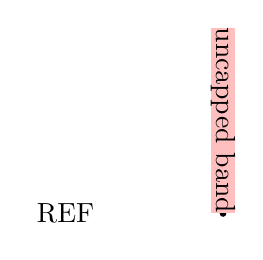
\begin{tikzpicture}[x=1cm,y=1cm]
  \node (A) at (-2,0) {REF};
  \fill (0,0) circle (1.2pt);
  \node[anchor=east,rotate=-90,fill=red!25,inner sep=0pt] at (0,0) {uncapped band};
\end{tikzpicture}
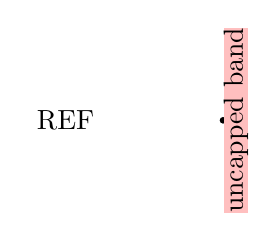
\begin{tikzpicture}[x=1cm,y=1cm]
  \node (A) at (-2,0) {REF};
  \fill (0,0) circle (1.2pt);
  \node[anchor=north,rotate=90,fill=red!25,inner sep=0pt] at (0,0) {uncapped band};
\end{tikzpicture}
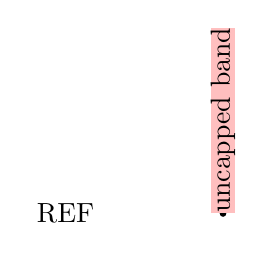
\begin{tikzpicture}[x=1cm,y=1cm]
  \node (A) at (-2,0) {REF};
  \fill (0,0) circle (1.2pt);
  \node[anchor=west,rotate=90,fill=red!25,inner sep=0pt] at (0,0) {uncapped band};
\end{tikzpicture}
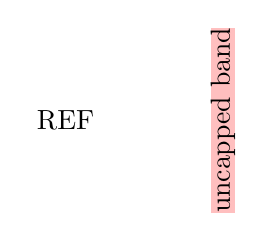
\begin{tikzpicture}[x=1cm,y=1cm]
  \node (A) at (-2,0) {REF};
  \fill (0,0) circle (1.2pt);
  \node[rotate=90,fill=red!25,inner sep=0pt] at (0,0) {uncapped band};
\end{tikzpicture}
\end{document}
